\documentclass{ClassePretiresCyberPunkRED}
%=========================== En-Tete =================================

\setmarginsrb{0.20cm}{0.20cm}{0.20cm}{0.20cm}{15pt}{3pt}{42pt}{15pt}
	
% --- style de page (pour les en-tete) ---
\pagestyle{empty}

% mettre du texte en diagonale sur le fond : tikz
\usepackage{tikz} 
\def\confidentialTIKZ{%
	\begin{tikzpicture}[remember picture,overlay]
	\node[rotate=60,scale=15,text opacity=0.1] at (current page.center) {Confidentiel};
	\end{tikzpicture}
}%

\def\TIKZcyberpunkRED{%
	\begin{tikzpicture}[remember picture,overlay]
	\node[rotate=60,scale=10,text opacity=0.1] at (current page.center) {-- Cyberpunk RED};
	\end{tikzpicture}
}%

\def\txtTITLE{Feuille de personnage Cyberpunk RED} %%%%% !! TITRE !! %%%%%
\def\imgCORNER{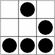
\includegraphics[width=0.25cm]{../../../images/glider/logo-glider.png}}

\def\imgGLIDERLEFTT{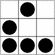
\includegraphics[width=1.95cm]{../../../images/glider/logo-glider-left.png}}
\def\imgGLIDERRIGHT{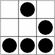
\includegraphics[width=1.95cm]{../../../images/glider/logo-glider-right.png}}

\def\imgGLIDERLEFTTsmall{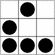
\includegraphics[width=0.25cm]{../../../images/glider/logo-glider-left.png}}
\def\imgGLIDERRIGHTsmall{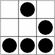
\includegraphics[width=0.25cm]{../../../images/glider/logo-glider-right.png}}

% % % en-tete et pieds de page configurables : fancyhdr.sty
\usepackage{fancyhdr}
\pagestyle{fancy}
	% \renewcommand{\chaptermark}[1]{\markboth{#1}{}}
	% \renewcommand{\sectionmark}[1]{\markright{\thesection\ #1}}
\fancyhf{}
\fancyhead[LE,RO]{\bfseries\thepage \TIKZcyberpunkRED }
\fancyhead[LO]{\bfseries\rightmark}
\fancyhead[RE]{\bfseries\leftmark}
\fancyfoot[LE]{\thepage /\pageref{LastPage} \hfill
	\scriptsize{\txtTITLE} % TITLE
\hfill \imgGLIDERLEFTTsmall }
\fancyfoot[RO]{\imgGLIDERRIGHTsmall \hfill
	\scriptsize{\txtTITLE} % TITLE
\hfill \thepage /\pageref{LastPage}}
\renewcommand{\headrulewidth}{0.5pt}
\renewcommand{\footrulewidth}{0.5pt}
\addtolength{\headheight}{0.5pt}
% \fancypagestyle{plain}{
	% \fancyhead{}
	% \renewcommand{\headrulewidth}{0pt}
% }

\def\smallbox{%
	\setlength{\unitlength}{0.5cm}
	\fbox{
		\begin{picture}(1, 1)(0,0)
		\end{picture}
	}
}%

%%%%%%%%%%% SOME VALUES IN ENGLISH %%%%%%%%%%%%%%%%%%%%%
%% \def\ENdefNom{\textbf{Name} \dotfill }

%============================= Corps =================================
\begin{document}
	
\setlength\parindent{0pt}

\begin{tabular}{ p{0.95\textwidth} }
	%% \CELLredTXTWhite
	\begin{tabular}{|p{0.20\linewidth}|p{0.75\linewidth}|} \hline
		\multirow{9}{*}{	%% \begin{tikzpicture}
							%% 	\node[maninblack,mirrored,monitor,saturated,minimum size=2.5cm]{A Corpo Rat ?};
							%% \end{tikzpicture}
							\newline \newline \newline \newline \newline \newline \newline \newline \newline 
		}
							&	\headerNameClass{RedEye NightCity}{NetRunner} %% \framebox[0.60\textwidth][ht]{ \newline \newline }	
												\\ \cline{2-2} 
							&	\begin{tabular}{|p{0.05\textwidth}|p{0.05\textwidth}|p{0.05\textwidth}|p{0.05\textwidth}|p{0.05\textwidth}|p{0.05\textwidth}|p{0.05\textwidth}|p{0.05\textwidth}|p{0.05\textwidth}|p{0.05\textwidth}|}
									\hline
									INT						&	REF						&	DEX						&	TECH					&	COOL					&	WILL					&	LUCK					&	MOVE					&	BODY					&	EMP						\\ \hline
									\CaracByFive{1}{2}{3}{4}{5}																												&	\CaracByFive{1}{2}{3}{4}{5}																												\\ \hline
									%% 						&							&							&							&							&							&							&							&							&							\\ \hline
									\CaracANYone{5}			&	\CaracANYone{5}			&	\CaracANYone{6}			&	\CaracANYone{6}			&	\CaracANYone{7}			&	\CaracANYone{7}			&	\CaracANYone{8}			&	\CaracANYone{8}			&	\CaracANYone{9}			&	\CaracANYone{9}			\\ \hline
								\end{tabular}	\\ \cline{2-2}
							&					\\ \cline{2-2}
							&	\begin{tabular}{|p{0.20\textwidth}|p{0.20\textwidth}|p{0.20\textwidth}|p{0.20\textwidth}|}
									Heal Points		&	Armor SP \newline (HEAD and BODY)	&	Net Actions		&	Rep lvl	\\
								\end{tabular}	\\ \cline{2-2}
							&	\begin{tabular}{|p{0.20\textwidth}|p{0.20\textwidth}|p{0.20\textwidth}|p{0.20\textwidth}|}
													&										&					&			\\
								\end{tabular}	\\ %% \cline{2-2}
							&	\begin{tabular}{|p{0.20\textwidth}|p{0.20\textwidth}|p{0.20\textwidth}|p{0.20\textwidth}|}
													&										&					&			\\
								\end{tabular}	\\ %% \cline{2-2}
							&	\begin{tabular}{|p{0.20\textwidth}|p{0.20\textwidth}|p{0.20\textwidth}|p{0.20\textwidth}|}
													&										&					&			\\ \cline{1-4} %% \hline
								\end{tabular}	\\ %% \cline{2-2}
							&					\\ \cline{2-2}
							&					\\ \cline{2-2}
							
							&					\\ \hline
	\multicolumn{2}{ c }{ } \\
							\hline
	\multicolumn{2}{ c }{
		\begin{tabular}{|p{0.30\textwidth}|p{0.30\textwidth}|p{0.30\textwidth}|} \hline
		STARTING HITS		&		SEROUSLY WOUNDED		&	DEATH SAVE			\\ \hline
						 	&						 		&						\\ \hline
		\end{tabular}
	} \\
							 \hline
	\end{tabular}~\\~\\
	
	\begin{tabular}{ p{0.50\linewidth} p{0.50\linewidth} } \hline
		\footnotesize
		\begin{tabular}{|p{0.23\linewidth}|p{0.20\linewidth}|p{0.20\linewidth}|p{0.20\linewidth}|} \hline
			\textsc{\textbf{Skills}}	&	\textbf{DEX}			&	\textbf{COOL}				&	\textbf{Special}	\\ \hline
			\textbf{INT}				&	Evasion \dotfill		&	Bribery \dotfill			&	Interface \dotfill	\\ \hline
			Perception \dotfill			&	Athletics \dotfill		&	Interrogation \dotfill		&	(NetRunner)			\\ \hline
			Tracking \dotfill			&	Stealth \dotfill		&	Persuasion \dotfill			&						\\ \hline
			Education \dotfill			&	Brawling \dotfill		&	\textbf{WILL}				&						\\ \hline
					 \dotfill			&	Melee Weapon \dotfill	&	Concentration \dotfill		&						\\ \hline
			Local Expert \dotfill		&	\textbf{TECH}			&	\textbf{EMP}				&						\\ \hline
			\textbf{REF}				&	Basic tech \dotfill		&	Conversation \dotfill		&						\\ \hline
			Marksmanship \dotfill		&	CyberTech \dotfill		&	Human P. \dotfill			&						\\ \hline	%% Human Perception
			Driving \dotfill			&	First Aid \dotfill		&	Instrument \dotfill			&						\\ \hline	%% Play Instrument
		\end{tabular}
			&	
		\begin{tabular}{|p{0.27\linewidth}|p{0.27\linewidth}|p{0.27\linewidth}|}  \hline
										&							&								\\ \hline
			\textsc{\textbf{ARMOR}}		&							&								\\ \hline
										&							&								\\ \hline
			\multicolumn{3}{ c }{ } \\
			\multicolumn{3}{ c }{ } \\ \hline 
										& \textsc{\textbf{NAME}}	& \textsc{\textbf{DAMAGE}}		\\ \hline
			\textsc{\textbf{WEAPONS}}	&							&								\\ \hline
										&							&								\\ \hline
										
		\end{tabular}	\\	
		\multicolumn{2}{ c }{ } \\
		\multicolumn{2}{ c }{ } \\
		\multicolumn{2}{ c }{ } \\
		\begin{tabular}{|p{0.30\linewidth}|p{0.50\linewidth}|} \hline
			\textsc{\textbf{Background}}	&	\resizebox{0.46\linewidth}{25pt}{
\includegraphics{../../../images/pixel.png}}	\\ \hline
			\textsc{\textbf{Motivation}}	&	\resizebox{0.46\linewidth}{25pt}{
\includegraphics{../../../images/pixel.png}}	\\ \hline
			\textsc{\textbf{Goals}}			&	\resizebox{0.46\linewidth}{25pt}{
\includegraphics{../../../images/pixel.png}}	\\ \hline
			\textsc{\textbf{Friends}}		&	\resizebox{0.46\linewidth}{25pt}{
\includegraphics{../../../images/pixel.png}}	\\ \hline
			\textsc{\textbf{Ennemies}}		&	\resizebox{0.46\linewidth}{25pt}{
\includegraphics{../../../images/pixel.png}}	\\ \hline
			\textsc{\textbf{Romance}}		&	\resizebox{0.46\linewidth}{25pt}{
\includegraphics{../../../images/pixel.png}}	\\ \hline
			\textsc{\textbf{Personnality}}	&	\resizebox{0.46\linewidth}{25pt}{
\includegraphics{../../../images/pixel.png}}	\\ \hline
			\multicolumn{2}{ c }{ } \\
			\multicolumn{2}{ c }{ } \\
			\multicolumn{2}{ c }{ } \\
			\multicolumn{2}{ c }{ } \\
			\multicolumn{2}{ c }{ } \\
			%% 								&	\resizebox{0.46\linewidth}{25pt}{
\includegraphics{../../../images/pixel.png}}	\\ 
		\end{tabular}
			&
		\begin{tabular}{|p{0.46\linewidth}|p{0.46\linewidth}|} \hline
			\textsc{\textbf{CYBERWARE}}											& \textsc{\textbf{GEAR}}		\\ \hline
				\resizebox{0.46\linewidth}{120pt}{
\includegraphics{../../../images/pixel.png}}	& 								\\ \hline
				\resizebox{0.46\linewidth}{120pt}{
\includegraphics{../../../images/pixel.png}}	& 								\\ \hline
		\end{tabular}	\\
	
	\end{tabular}
\end{tabular}

\end{document}
